\chapter{Calibration du modèle} 

\lettrine{I}{l} est question ici de définir la méthodologie afin de calibrer les paramètres libres du modèle.
On s'intéressera notamment à définir une fonction de coût, pour évaluer la qualité de la calibration.
Dans cette optique, on essayera de calibrer les paramètres en utilisant uniquement les dynamiques du verger n\textdegree1 ; le deuxième servira à la validation.

Il peut être utile de donner la liste des paramètres à calibrer :
\begin{itemize}
 \item $\gamma$, le paramètre relatif à l'arrivée des femelles exogènes ;
 \item $p_{\text{m}}$, le paramètre relatif à la migration des femelles endogènes entre les sous-parcelles ;
 \item $\mu^{1}_{\text{ER}}$ et $\mu^{2}_{\text{ER}}$, les probabilité de réussir à entrer et à sortir du sol pour les cécidomyies pour la modalité «enherbement ras». Pour simplifier,
 on pose $\mu^{1}_{\text{ER}} = \mu^{2}_{\text{ER}}$;
 \item $\mu^{1}_{\text{EH}}$ et $\mu^{2}_{\text{EH}}$, les probabilité de réussir à entrer et à sortir du sol pour les cécidomyies pour la modalité «enherbement haut». Ici aussi,
 on pose $\mu^{1}_{\text{EH}} = \mu^{2}_{\text{EH}}$;
 \item $k$, le paramètre relatif à la disponibilité en ressources pour les inflorescences ;
 \item \texttt{stock}, le nombre de larves entrées en diapause les années précédentes qui décident de sortir l'année considérée ;
 \item $E_0\mu_{\ell}$, le nombre d'œufs pondus par une femelle qui survivent, se transforment en larves puis s'éjectent de l'inflorescences. 
\end{itemize}


\section{Fonction de coût}

Avant une quelconque estimation des paramètres, nous avons besoin de mesurer la qualité de nos estimations.
Pour ce faire, on utilisera une fonction pour comparer le nombre de larves estimées avec le nombre de larves observées. 
Pour définir cette fonction, on pose :
\begin{itemize}
 \item $m$, le nombre de jours entre la première observation et la dernière ;
 \item $n$, le nombre de relevés effectif;
 \item $t$, le nombre de jours passés depuis la première observation ;
 \item $t^j$, le nombre de jours entre la première observation et le $j^{\text{ème}}$ relevé.
\end{itemize}
(On a donc $t^1 = 0$ et $t^n = m$.)

La fonction est alors définie par
$$
f(y, \hat y) = \frac{\sqrt{\frac{1}{n-1}\sum_{j=2}^n\left( y^*_j - \hat y^*_j \right)^2}}{\max(y^*) - \min(y^*)},
$$
où 
$$y^*_j =  y_{t^j} \qquad \text{ et } \qquad \hat y^*_j = \frac{1}{t^j - t^{j-1}}\sum_{k=t^{j-1}}^{t^j} \hat y_k.$$
La figure~\ref{fig:calib} illustre le fonctionnement de la fonction.
Appliquer la fonction à $n-1$ valeurs (correspondant aux relevés sur le terrain) plutôt qu'à chacun des $m$ jours (correspondant à l'étendue des relevés) est motivé par le fait que les relevés ne furent pas fait à des intervalles de temps régulier.
Ce faisant, on évite d'attribuer plus d'importance aux relevés qui ont eu un écart relativement important avec le relevé précédent.

\begin{figure}[ht]
\centering
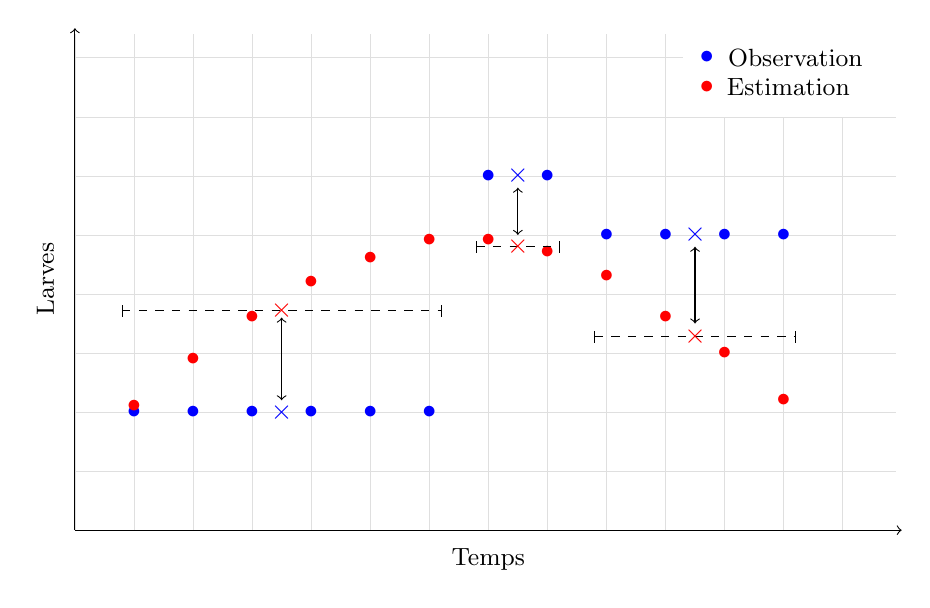
\begin{tikzpicture}[scale = 0.75]
 \draw [very thin, lightgray, opacity = 0.5] (0,0) grid (13.9, 8.4);
 \draw [->] (0, 0) -- (0, 8.5);
 \draw [->] (0, 0) -- (14, 0);
 \draw (1, 2) node{\textcolor{blue}{$\bullet$}};
 \draw (2, 2) node{\textcolor{blue}{$\bullet$}};
 \draw (3, 2) node{\textcolor{blue}{$\bullet$}};
 \draw (4, 2) node{\textcolor{blue}{$\bullet$}};
 \draw (5, 2) node{\textcolor{blue}{$\bullet$}};
 \draw (6, 2) node{\textcolor{blue}{$\bullet$}};
 \draw (7, 6) node{\textcolor{blue}{$\bullet$}};
 \draw (8, 6) node{\textcolor{blue}{$\bullet$}};
 \draw (9 , 5) node{\textcolor{blue}{$\bullet$}};
 \draw (10, 5) node{\textcolor{blue}{$\bullet$}};
 \draw (11, 5) node{\textcolor{blue}{$\bullet$}};
 \draw (12, 5) node{\textcolor{blue}{$\bullet$}};
 \draw (1, 2.1) node{\textcolor{red}{$\bullet$}};
 \draw (2, 2.9) node{\textcolor{red}{$\bullet$}};
 \draw (3, 3.6) node{\textcolor{red}{$\bullet$}};
 \draw (4, 4.2) node{\textcolor{red}{$\bullet$}};
 \draw (5, 4.6) node{\textcolor{red}{$\bullet$}};
 \draw (6, 4.9) node{\textcolor{red}{$\bullet$}};
 \draw (7, 4.9) node{\textcolor{red}{$\bullet$}};
 \draw (8, 4.7) node{\textcolor{red}{$\bullet$}};
 \draw (9, 4.3) node{\textcolor{red}{$\bullet$}};
 \draw (10, 3.6) node{\textcolor{red}{$\bullet$}};
 \draw (11, 3) node{\textcolor{red}{$\bullet$}};
 \draw (12, 2.2) node{\textcolor{red}{$\bullet$}};
 \draw [dashed] (0.8, 3.716) -- (6.2, 3.716) ;
 \draw [dashed] (6.8, 4.8) -- (8.2, 4.8) ;
 \draw [dashed] (8.8, 3.275) -- (12.2, 3.275) ;
 \draw (0.8, 3.616) -- (0.8, 3.816);
 \draw (6.2, 3.616) -- (6.2, 3.816);
 \draw (6.8, 4.7) -- (6.8, 4.9);
 \draw (8.2, 4.7) -- (8.2, 4.9);
 \draw (8.8, 3.175) -- (8.8, 3.375);
 \draw (12.2, 3.175) -- (12.2, 3.375);
 \draw (3.5, 3.716) node{\textcolor{red}{$\times$}};
 \draw (7.5, 4.8) node{\textcolor{red}{$\times$}}; 
 \draw (10.5, 3.275) node{\textcolor{red}{$\times$}};
 \draw (3.5, 2) node{\textcolor{blue}{$\times$}};
 \draw (7.5, 6) node{\textcolor{blue}{$\times$}}; 
 \draw (10.5, 5) node{\textcolor{blue}{$\times$}}; 
 \draw [<->] (3.5, 2.2) -- (3.5, 3.6);                  
 \draw [<->] (7.5, 5.8) -- (7.5, 5);
 \draw [<->] (10.5, 4.8) -- (10.5, 3.5);
 \draw [fill=white,white] (10.3, 7.01) rectangle (13.9, 8.4);
 \draw (12.2, 8) node {{\small Observation}};
 \draw (12.08, 7.5) node {{\small Estimation}};
 \draw (10.7, 8) node{\textcolor{blue}{$\bullet$}};
 \draw (10.7, 7.5) node{\textcolor{red}{$\bullet$}};
 \draw (6, 0.135) node[rotate = 180] {\textcolor{ForestGreen}{$\intercal$}};
 \draw (8, 0.135) node[rotate = 180] {\textcolor{ForestGreen}{$\intercal$}};
 \draw (12, 0.135) node[rotate = 180] {\textcolor{ForestGreen}{$\intercal$}};
 \draw (7, -0.5) node{\small \text{Temps}};
 \draw  (-0.5, 4.25) node{\rotatebox{90}{\small Larves}};
\end{tikzpicture}
\caption{Schéma illustrant le fonctionnement de la fonction objectif. À chaque relevé effectif (marqueurs verts), on fait correspondre la période correspondant à ce relevé (segments en pointillés).
Et pour chacune de ces périodes, on calcule la moyenne des valeurs estimées (les croix rouges). On compare ensuite les moyennes ainsi calculées avec les valeurs observées associées (les croix bleues).}
\label{fig:calib}
\end{figure}


Par la suite, l'objectif sera de minimiser cette fonction pour chacune des trois sous-parcelles.

\section{Analyse de sensibilité}

Avant de calibrer le modèle, il est pertinent d'effectuer une analyse de sensibilité.
L'analyse de sensibilité est définie par \citet{saltelli2004} comme
\begin{quote}
 «l'étude de comment l'incertitude de la sortie d'un modèle --- qu'elle soit numérique ou non --- peut être répartie entre les différentes sources d'incertitudes présentes dans les entrées du modèle.»\footnote{«The study of how uncertainty in the output of a model (numerical or otherwise) can be apportioned to different sources of uncertainty in the model input.»}
\end{quote}
Autrement dit, on cherche à connaître les paramètres les plus influants sur la sortie du modèle.
La calibration comportant toujours une part d'arbitraire, cette analyse permet de prendre du recul sur les choix de paramètres, relativement à leur impact sur le modèle.
En particulier lorsque certains paramètres ne sont qu'approximatifs vis à vis de la réalité qu'ils ont vocation à décrire, mais fortement significatifs pour la sortie du modèle.

Il existe deux grandes catégories d'analyses de sensibilité, celles qui ont une approche globale et celles qui ont une approche locale (parfois appelées \emph{one-at-the-time}).
L'approche locale consiste à étudier la sensibilité des paramètres les uns après les autres, les uns indépendamment des autres.
Cette approche est valable si et seulement si le modèle est linéaire par rapport à chacune de ses entrées $x_i$ et qu'il n'y a aucune interaction entre les différentes entrées du modèle \citep{saltelli2019so}.
Dès lors qu'il y a la moindre incertitude sur la linéarité du modèle ou sur la non-interaction entre les paramètres, il faut privilégier une approche globale.
Notre modèle n'est pas linéaire et il n'y a dans notre cas aucune raison de supposer la non-interaction entre nos paramètres, bien au contraire.
On utilisera donc une approche globale.

Bien qu'il existe plusieurs méthodes ayant une approche globale, elles ont toutes en commun de fonctionner dans un cadre non-linéaire et de prendre en compte les différentes interactions entre les différents paramètres.
Parmi les méthodes les plus connues et les plus utilisées, on peut en citer qui fonctionnent par décomposition de la variance comme Sobol ou FAST (Fourier Amplitude Sensitivity Test) ou d'autres qui fonctionnent en effectuant des perturbations élémentaires des entrées du modèle comme la méthode Morris.
Notre modèle possède moins de 20 paramètres et s'exécute en moins d'une minute, nous utiliserons alors la méthode Sobol conformément aux recommendations de \citet[chap. 6]{saltelli}.

Le fonctionnement de cette méthode est relativement intuitif.
On considère que la sortie de notre modèle $Y$ peut s'exprimer comme une fonction des entrées de notre modèle $X,$ c'est-à-dire $Y = f(X)$.
Comme $X = \left( X_1, \ldots, X_n \right)$ peut prendre plein de valeurs possibles, il en résulte qu'il y a \emph{a priori} plein de résultats possibles pour $Y.$
% L'objectif est alors de décomposer ces résultats possibles --- cette variance qu'admet $Y$ --- en fonction de chaque entrée du modèle $X_i$.
L'objectif est alors de déterminer quelles entrées du modèle $X_i$ induisent le plus de changements dans ces résultats possibles --- dans cette variance qu'admet $Y.$
À cette fin, on utilise les indices pricipaux de Sobol définis par
\[
S_i = \frac{\textbf{Var}\!\left( \mathbf{E}\!\left[Y|X_i\right] \right)}{\textbf{Var}\!\left( Y \right)}.
\]
% L'indice $S_i$ permet de voir l'effet du seul paramètre $X_i$ sur la variance de $Y$ relativement aux autres.
Ici, $\textbf{Var}\!\left( \mathbf{E}\left[Y|X_i\right] \right)$ permet de voir l'effet du seul paramètre $X_i$ sur la variance de $Y.$
Diviser par la variance totale de $Y$ permet de le faire relativement aux autres paramètres.
Cet indice ne prend cependant pas en compte les interactions entre $X_i$ et les autres entrées du modèle. 
Il faut pour ça utiliser les indices totaux de Sobol définis par
\[
S^T_i = 1 - \frac{\textbf{Var}\!\left( \mathbf{E}\!\left[Y|X_{\sim i}\right] \right)}{\textbf{Var}\!\left( Y \right)},
\]
où $X_{\sim i} = \left(X_1, \ldots, X_{i-1}, X_{i+1}, \ldots, X_n \right)$.
L'indice $S^T_i$ ainsi défini permet lui de prendre en compte l'impact du paramètre $X_i$ et de ses interactions sur la variance de $Y$.
À noter que l'interaction entre $X_i$ et $X_j$ est à la fois prise en compte par $S^T_i$ et $S^T_j$.
C'est pour cette raison qu'il est souvent pertinent d'interpréter les indices principaux et les indices totaux conjointement.

Une fois que l'on connaît la sensibilité du modèle aux différents paramètres, on peut alors passer à la calibration desdits paramètres.


\section{Algorithme d'optimisation}

L'objectif de l'optimisation est de trouver les jeux de paramètres qui minimisent notre fonction de coût, ceux qui permettent d'ajuster au mieux les dynamiques de larves simulées aux dynamiques observées.
Pour ce faire, on a besoin d'un algorithme d'optimisation.
Et il y a du choix.

On peut déjà noter que nous avons sept paramètres à calibrer, et qu'ils évoluent tous dans des intervalles (que l'on définira plus tard).
Il apparaît évident que toutes les solutions ne pourront pas être testées.
Une solution peut être d'utiliser un algorithme basé sur une méthode MCMC comme l'algorithme du recuit simulé.
Nous avons cependant trois dynamiques à ajuster (une pour chaque sous-parcelle), il faudrait alors minimiser la somme (ou la moyenne) des trois fonctions objectifs.
Ou alors on peut directement utiliser un algorithme d'optimisation multicritères.

Ces algorithmes ont l'avantage de pouvoir optimiser simultanément des objectifs qui ne sont pas toujours comparables --- à des échelles différentes, par exemple.
Un des plus connus est sans conteste NSGA-II (Nondominated Sorting Genetic Algorithm II) \citep{deb}.
C'est celui que l'on utilisera.

C'est un algorithme qui ne renvoie pas une unique solution mais un ensemble de solutions. 
Cet ensemble de solutions converge vers un sous-ensemble du front de Pareto.
Le front de Pareto désigne l'ensemble des solutions non-dominées pour un problème donné.
Dans $P \subset \mathbf{R}^{p}$ ($n$ > 1), une solution $x = \left( x_1, \ldots, x_p \right) \in  P$ est dite non-dominée lorsque
\[
\left\{ y \in P\ |\ \forall\ i \in \{1, \ldots, p\},\ y_i \succcurlyeq x_i \text{ et } \exists\ i \text{ tel que } y_i \succ x_i \right\} = \emptyset,
\]
où $\succcurlyeq$ et $\succ$ veulent respectivement dire «au moins aussi bien que» et «meilleur que». 
Dans notre cas, vu que l'on veut minimiser notre fonction de coût, $\succcurlyeq$ se traduira par $\leq$ et $\succ$ se traduira par $<$.
En d'autres termes, $x$ est non-dominée signifie qu'il n'existe pas de solution $y$ qui soit strictement meilleure sur un des critères et au moins aussi bonne sur tous les autres critères.

Le front de Pareto étant un sous-ensemble de $\mathbf{R}^{p}$, il n'est (\emph{a priori}) pas dénombrable.
De ce fait, NSGA-II ne peut pas renvoyer le front tout entier mais seulement un sous-ensemble.
C'est un algorithme itératif, les itérations seront appelées ici \emph{générations}.
Et il faut plusieurs générations pour se retrouver avec des solutions non-dominées.
À la génération $t$, l'algorithme effectue plusieurs opérations.
\begin{enumerate}
 \item On possède un ensemble de solutions potentielles que l'on nommera \emph{population}.
 La taille de la population $N$ est fixée arbitrairement.
 \item À chaque solution de cette population $P_t$, on attribue une solution fille (on verra plus tard comment). 
\end{enumerate}

 Avec la population $P_t$ et les solutions filles associées $F_t$, cela forme un ensemble de solutions potentielles $S_t$ de taille $2N$. 
 On va alors sélectionner parmi ces solutions les $N$ solutions qui nous intéressent le plus.
\begin{enumerate}[resume]
 \item Pour ce faire, pour chaque solution potentielle $s\in S_t$ :
 \begin{itemize}
  \item on calcule le nombre $n_s$ d'éléments de $S_t$ qui domine qui domine $s$ ;
  \item on établit l'ensemble $D_s$ des autres solutions de $S_t$ qui sont dominées par la solution $s$.
 \end{itemize}
 \item On répartit alors nos solutions en plusieurs groupes, en plusieurs \emph{fronts}.
 Vont ainsi dans le premier front $F_1$ les solutions $s$ qui vérifient $n_s = 0$, qui ne sont donc pas dominées par d'autres solutions de $S_t$. 
 Dans le deuxième front $F_2$ se trouvent les solutions qui sont dominées uniquement par les solutions présentes dans $F_1$.
 (Autrement dit, les solutions qui se trouvent dans et uniquement dans $\bigcup_{s\in F_1} D_s$.)
 On continue de la même manière pour $F_3$ (qui contient les solutions uniquement dominées par celles de $F_1$ et $F_2$), $F_4$... jusqu'à ce que toutes les solutions de $S_t$ soient assignées à un front.
 \item On choisira alors de garder en priorité les solutions de $F_1$ puis de $F_2$ et ainsi de suite jusqu'à en obtenir $N$. 
 Il faut noter qu'il existe probablement un front $F_k$ où toutes les solutions ne pourront être garger pour ne pas dépasser la limite imposée de $N$ solutions.
 Plutôt que de choisir aléatoirement le nombre nécésaires de solutions dans $F_k$, seront sélectionnées les solutions qui maximisent une certaine distance --- the \emph{crowding distance} --- avec les autres solutions.
 (On n'entrera pas dans le détail ici.)
 C'est fait pour assurer une certaine diversité entre les différentes solutions.
 Les $N$ solutions ainsi sélectionnées constitueront $P_{t+1}$, la population initiale de la génération suivante $t+1$.
\end{enumerate}

Un élément important pour assurer une convergence vers le front de Pareto est le choix des solutions filles $F_t$ effectué à chaque génération.
Pour générer une solution fille, plusieurs étapes sont là aussi nécessaires.
Ces étapes (simplifiées) sont :
\begin{enumerate}
 \item On selectionne deux solutions $s_1$ et $s_2$ dans $P_t$.
 \item On construit une solution fille $f_1$ en prenant la moitié des coordonnées de $s_1$ et l'autre moitié de $s_2$. 
 On construit $f_2$ en prenant les moitiés de $s_1$ et $s_2$ inutilisées dans la construction de $f_1$.
 \item Sur chacune des solutions filles, une coordonnée choisie aléatoirement est remplacée par une valeur aléatoire choisie dans un intervalle centré sur la valeur initiale.
 \item On réitère ces étapes jusqu'à avoir $N$ solutions filles.
\end{enumerate}


Et c'est ainsi qu'après un nombre suffisant d'itérations, et pour une taille de population suffisament grande, l'algorithme NSGA-II renvoie un ensemble de points suffisament proche du front de Pareto et qui en retranscrit sa diversité.


Dans notre cas, cela signifie que l'on possède différents jeux de paramètres et les valeurs de la fonction de coût pour les trois sous-blocs qu'ils produisent.
Et qu'il ne reste plus qu'à faire un choix.



\section{Exploration de l'ensemble des solutions}


Choisir une solution n'est cependant pas trivial.
En effet, parmi les solutions possibles, aucune n'est objectivement meilleure que les autres.
Il en découle que le choix sera forcément arbitraire.

Plusieurs approches sont possibles.
On peut par exemple choisir au hasard un nombre restreint de solutions possibles, les tester puis sélectionner celle qui semble la plus pertinente.
On peut aussi sélectionner la solution associée aux trois critères qui minimisent une distance à 0, en estimant qu'elle représente un bon compromis entre les différents critères.

Ou alors on essaye d'avoir une vision globale de l'ensemble des solutions.
Il peut même être pertinent de comprendre voire d'\emph{expliquer} quel jeu de paramètres génère quelle solution.
Le choix du jeu de paramètre sera alors plus réfléchi, bien que toujours arbitraire.

Plus précisément, on possède les valeurs de la fonction de coût de nos critères rassemblées dans un tableau $Y$.
On possède également les jeux de paramètres (nos solutions) responsables de ces valeurs rassemblés dans un tableau $X$.
Le but serait alors d'explorer $Y,$ pour savoir par exemple si les critères sont antagonistes (\emph{e.g.} améliorer la prédiction sur une sous-parcelle ne détériore pas la solution de la sous-parcelle voisine ?) ou alors totalement indépendant.
Mais aussi de pouvoir dire quelles sont les valeurs pour les variables de $X$ qui minimisent quel critère de $Y$. 
À cette fin, on peut choisir entre deux méthodes : l'ACP-VI  et la régression PLS2.
